\documentclass[journal,12pt,twocolumn]{IEEEtran}
\usepackage{setspace}
\usepackage{gensymb}
\usepackage{caption}
%\usepackage{multirow}
%\usepackage{multicolumn}
%\usepackage{subcaption}
%\doublespacing
\singlespacing
\usepackage{csvsimple}
\usepackage{amsmath}
\usepackage{multicol}
%\usepackage{enumerate}
\usepackage{amssymb}
%\usepackage{graphicx}
\usepackage{newfloat}
%\usepackage{syntax}
\usepackage{listings}
\usepackage{iithtlc}
\usepackage{color}
\usepackage{tikz}
\usetikzlibrary{shapes,arrows}



%\usepackage{graphicx}
%\usepackage{amssymb}
%\usepackage{relsize}
%\usepackage[cmex10]{amsmath}
%\usepackage{mathtools}
%\usepackage{amsthm}
%\interdisplaylinepenalty=2500
%\savesymbol{iint}
%\usepackage{txfonts}
%\restoresymbol{TXF}{iint}
%\usepackage{wasysym}
\usepackage{amsthm}
\usepackage{mathrsfs}
\usepackage{txfonts}
\usepackage{stfloats}
\usepackage{cite}
\usepackage{cases}
\usepackage{mathtools}
\usepackage{caption}
\usepackage{enumerate}	
\usepackage{enumitem}
\usepackage{amsmath}
%\usepackage{xtab}
\usepackage{longtable}
\usepackage{multirow}
%\usepackage{algorithm}
%\usepackage{algpseudocode}
\usepackage{enumitem}
\usepackage{mathtools}
\usepackage{hyperref}
%\usepackage[framemethod=tikz]{mdframed}
\usepackage{listings}
    %\usepackage[latin1]{inputenc}                                 %%
    \usepackage{color}                                            %%
    \usepackage{array}                                            %%
    \usepackage{longtable}                                        %%
    \usepackage{calc}                                             %%
    \usepackage{multirow}                                         %%
    \usepackage{hhline}                                           %%
    \usepackage{ifthen}                                           %%
  %optionally (for landscape tables embedded in another document): %%
    \usepackage{lscape}     


\usepackage{url}
\def\UrlBreaks{\do\/\do-}


%\usepackage{stmaryrd}


%\usepackage{wasysym}
%\newcounter{MYtempeqncnt}
\DeclareMathOperator*{\Res}{Res}
%\renewcommand{\baselinestretch}{2}
\renewcommand\thesection{\arabic{section}}
\renewcommand\thesubsection{\thesection.\arabic{subsection}}
\renewcommand\thesubsubsection{\thesubsection.\arabic{subsubsection}}

\renewcommand\thesectiondis{\arabic{section}}
\renewcommand\thesubsectiondis{\thesectiondis.\arabic{subsection}}
\renewcommand\thesubsubsectiondis{\thesubsectiondis.\arabic{subsubsection}}

% correct bad hyphenation here
\hyphenation{op-tical net-works semi-conduc-tor}

%\lstset{
%language=C,
%frame=single, 
%breaklines=true
%}

%\lstset{
	%%basicstyle=\small\ttfamily\bfseries,
	%%numberstyle=\small\ttfamily,
	%language=Octave,
	%backgroundcolor=\color{white},
	%%frame=single,
	%%keywordstyle=\bfseries,
	%%breaklines=true,
	%%showstringspaces=false,
	%%xleftmargin=-10mm,
	%%aboveskip=-1mm,
	%%belowskip=0mm
%}

%\surroundwithmdframed[width=\columnwidth]{lstlisting}
\def\inputGnumericTable{}                                 %%
\lstset{
%language=C,
frame=single, 
breaklines=true,
columns=fullflexible
}
 

\begin{document}
%
\tikzstyle{block} = [rectangle, draw,
    text width=3em, text centered, minimum height=3em]
\tikzstyle{sum} = [draw, circle, node distance=3cm]
\tikzstyle{input} = [coordinate]
\tikzstyle{output} = [coordinate]
\tikzstyle{pinstyle} = [pin edge={to-,thin,black}]

\theoremstyle{definition}
\newtheorem{theorem}{Theorem}[section]
\newtheorem{problem}{Problem}
\newtheorem{proposition}{Proposition}[section]
\newtheorem{lemma}{Lemma}[section]
\newtheorem{corollary}[theorem]{Corollary}
\newtheorem{example}{Example}[section]
\newtheorem{definition}{Definition}[section]
%\newtheorem{algorithm}{Algorithm}[section]
%\newtheorem{cor}{Corollary}
\newcommand{\BEQA}{\begin{eqnarray}}
\newcommand{\EEQA}{\end{eqnarray}}
\newcommand{\define}{\stackrel{\triangle}{=}}

\bibliographystyle{IEEEtran}
%\bibliographystyle{ieeetr}

\providecommand{\nCr}[2]{\,^{#1}C_{#2}} % nCr
\providecommand{\nPr}[2]{\,^{#1}P_{#2}} % nPr
\providecommand{\mbf}{\mathbf}
\providecommand{\pr}[1]{\ensuremath{\Pr\left(#1\right)}}
\providecommand{\qfunc}[1]{\ensuremath{Q\left(#1\right)}}
\providecommand{\sbrak}[1]{\ensuremath{{}\left[#1\right]}}
\providecommand{\lsbrak}[1]{\ensuremath{{}\left[#1\right.}}
\providecommand{\rsbrak}[1]{\ensuremath{{}\left.#1\right]}}
\providecommand{\brak}[1]{\ensuremath{\left(#1\right)}}
\providecommand{\lbrak}[1]{\ensuremath{\left(#1\right.}}
\providecommand{\rbrak}[1]{\ensuremath{\left.#1\right)}}
\providecommand{\cbrak}[1]{\ensuremath{\left\{#1\right\}}}
\providecommand{\lcbrak}[1]{\ensuremath{\left\{#1\right.}}
\providecommand{\rcbrak}[1]{\ensuremath{\left.#1\right\}}}
\theoremstyle{remark}
\newtheorem{rem}{Remark}
\newcommand{\sgn}{\mathop{\mathrm{sgn}}}
\providecommand{\abs}[1]{\left\vert#1\right\vert}
\providecommand{\res}[1]{\Res\displaylimits_{#1}} 
\providecommand{\norm}[1]{\lVert#1\rVert}
\providecommand{\mtx}[1]{\mathbf{#1}}
\providecommand{\mean}[1]{E\left[ #1 \right]}
\providecommand{\fourier}{\overset{\mathcal{F}}{ \rightleftharpoons}}
%\providecommand{\hilbert}{\overset{\mathcal{H}}{ \rightleftharpoons}}
\providecommand{\system}{\overset{\mathcal{H}}{ \longleftrightarrow}}
	%\newcommand{\solution}[2]{\textbf{Solution:}{#1}}
\newcommand{\solution}{\noindent \textbf{Solution: }}
\newcommand{\myvec}[1]{\ensuremath{\begin{pmatrix}#1\end{pmatrix}}}
\providecommand{\dec}[2]{\ensuremath{\overset{#1}{\underset{#2}{\gtrless}}}}
\DeclarePairedDelimiter{\ceil}{\lceil}{\rceil}
%\numberwithin{equation}{subsection}
%\numberwithin{equation}{section}
%\numberwithin{problem}{subsection}
%\numberwithin{definition}{subsection}
\makeatletter
\@addtoreset{figure}{section}
\makeatother

\let\StandardTheFigure\thefigure
%\renewcommand{\thefigure}{\theproblem.\arabic{figure}}
\renewcommand{\thefigure}{\thesection}


%\numberwithin{figure}{subsection}

%\numberwithin{equation}{subsection}
%\numberwithin{equation}{section}
%\numberwithin{equation}{problem}
%\numberwithin{problem}{subsection}
\numberwithin{problem}{section}
%%\numberwithin{definition}{subsection}
%\makeatletter
%\@addtoreset{figure}{problem}
%\makeatother
\makeatletter
\@addtoreset{table}{section}
\makeatother

\let\StandardTheFigure\thefigure
\let\StandardTheTable\thetable
\let\vec\mathbf
%%\renewcommand{\thefigure}{\theproblem.\arabic{figure}}
%\renewcommand{\thefigure}{\theproblem}

%%\numberwithin{figure}{section}

%%\numberwithin{figure}{subsection}



\def\putbox#1#2#3{\makebox[0in][l]{\makebox[#1][l]{}\raisebox{\baselineskip}[0in][0in]{\raisebox{#2}[0in][0in]{#3}}}}
     \def\rightbox#1{\makebox[0in][r]{#1}}
     \def\centbox#1{\makebox[0in]{#1}}
     \def\topbox#1{\raisebox{-\baselineskip}[0in][0in]{#1}}
     \def\midbox#1{\raisebox{-0.5\baselineskip}[0in][0in]{#1}}

\vspace{3cm}

\title{ 
	\logo{
Python with Linear Algebra: 2D 
	}
}

\author{ G V V Sharma$^{*}$% <-this % stops a space
	\thanks{*The author is with the Department
		of Electrical Engineering, Indian Institute of Technology, Hyderabad
		502285 India e-mail:  gadepall@iith.ac.in. All content in this manual is released under GNU GPL.  Free and open source.}
	
}	

\maketitle

\tableofcontents

\bigskip

\renewcommand{\thefigure}{\theenumi}
\renewcommand{\thetable}{\theenumi}

\begin{abstract}
This manual introduces matrix computations using python and the properties of a triangle.
\end{abstract}
\section{Line}
\begin{enumerate}[label=\thesection.\arabic*
,ref=\thesection.\theenumi]
%
\item
\label{prob:draw_triangle}
Let
\begin{equation}
\vec{A} =
\myvec{-2\\-2},
\vec{B} =
\myvec{1\\3},
\vec{C} =
\myvec{4\\-1},
\end{equation}
%
Find the direction vector and the normal vector for $AB$
\\
\solution 
%Let
%\begin{align}
%T_{AB} = \myvec{\vec{A} & \vec{B}} = \myvec{-2 & 1\\ -2 & 3}
%\end{align}
The direction vector of $AB$ is 
\begin{align}
\label{eq:dir_vec}
\vec{m} &= \vec{B}-\vec{A} 
\\
&=  
\myvec{1 \\ 3} - \myvec{-2\\-2}
\\
&= \myvec{1-(-2)\\3-(-2)}=\myvec{3\\5}
\end{align}
%
\item Find the {\em normal} vector of $AB$.
\\
\solution The normal vector $\vec{n}$ is defined as
\begin{align}
\label{eq:line_nor}
\vec{n}^T\vec{m} &= 0
\end{align}
and can be obtained as
\begin{align}
\vec{n}&= \myvec{0 & 1 \\ -1 & 0}\vec{m} 
\\
&=\myvec{0 & 1 \\ -1 & 0}\myvec{3\\5}
\\
&= \myvec{0\times 3 + 1 \times 5  \\ -1\times 3 + 0 \times 5}=\myvec{5\\-3}
\end{align}
\item Verify \eqref{eq:line_nor}.
\\
\solution 
\begin{align}
\vec{n}^T\vec{m} &= \myvec{5\\-3}^T\myvec{3\\5} = \myvec{5 & -3}\myvec{3\\5}
\\
 &= 5 \times 3 + (-3)\times 5 = 0 
\end{align}
\item Find the equation of $AB$.
\\
\solution  The desired equation is obtained as
\begin{align}
\label{eq:line_dir}
\quad \vec{x} &= \vec{A}+ \lambda \brak{\vec{B}-\vec{A}}
\\
&= -\myvec{2\\2}+ \lambda\myvec{3\\5}
\end{align}
%
\item Draw the line $AB$
\\
\solution The following code plots $AB$ in Fig. \ref{fig:draw_line}
\lstinputlisting[language=python]{./codes/draw_line.py}
%
\begin{figure}
\centering
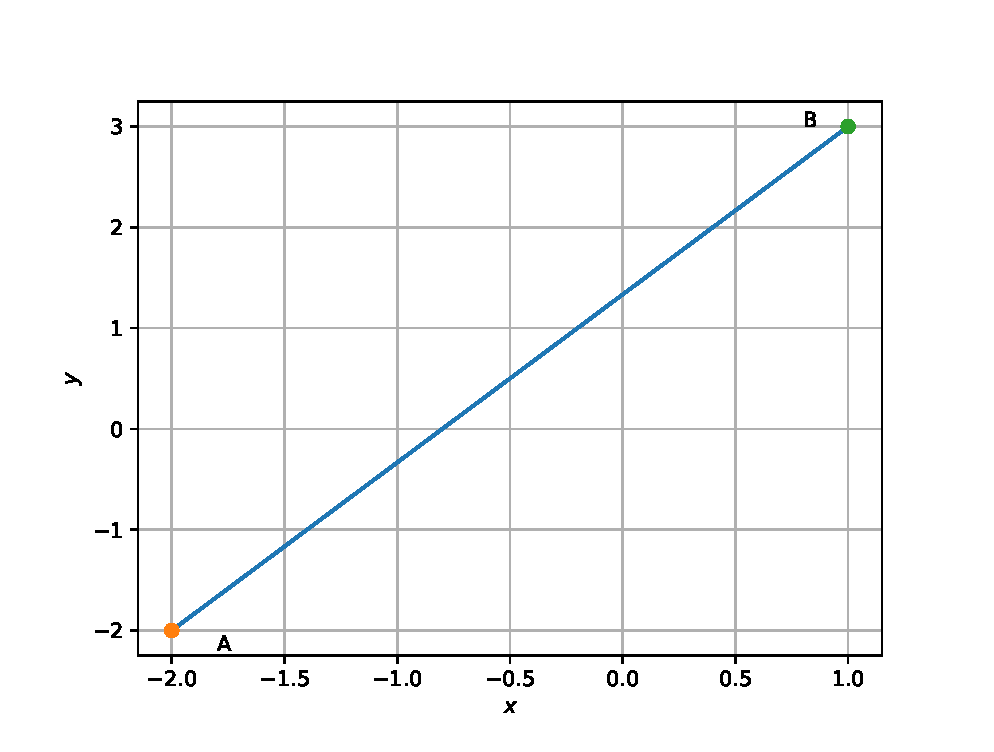
\includegraphics[width=\columnwidth]{./figs/draw_line.eps}
\caption{}
\label{fig:draw_line}
\end{figure}

\item Draw $\triangle ABC$.
\\
\solution
The following codes yields the desired plot in Fig. \ref{fig:triangle_def}
\begin{lstlisting}
https://raw.githubusercontent.com/gadepall/school/master/linalg/2D/python_2d/codes/coeffs.py
\end{lstlisting}
\begin{lstlisting}
https://raw.githubusercontent.com/gadepall/school/master/linalg/2D/python_2d/codes/draw_triangle.py
\end{lstlisting}

%\lstinputlisting{./codes/draw_triangle.py}

\begin{figure}
\centering
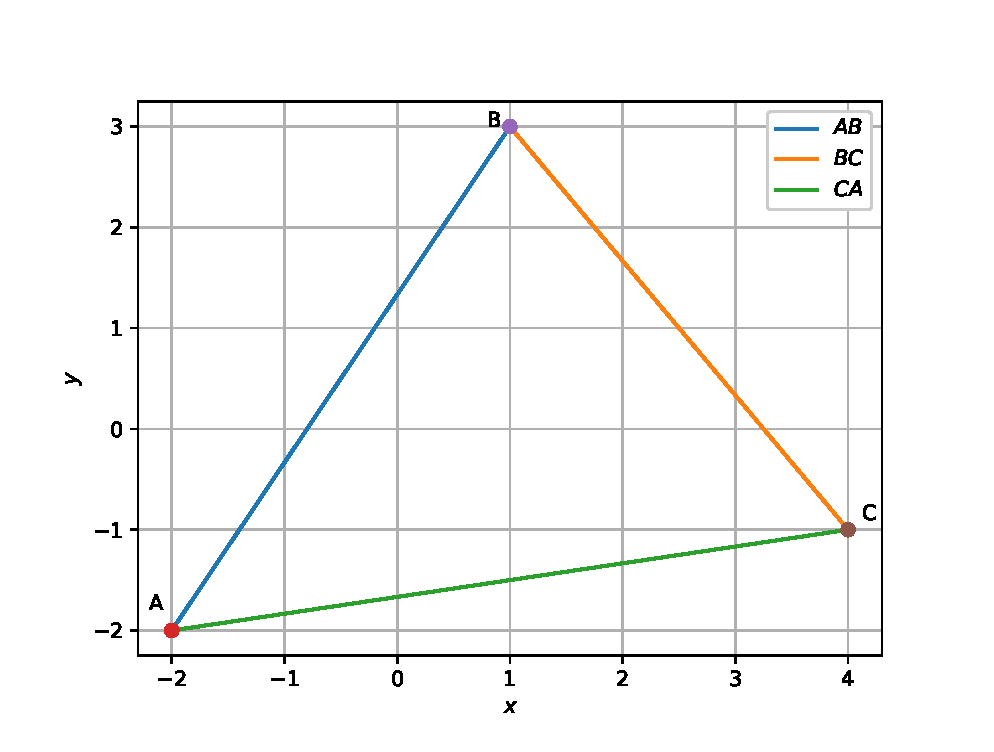
\includegraphics[width=\columnwidth]{./figs/triangle.eps}
\caption{}
\label{fig:triangle_def}
\end{figure}

%\item Write a python code for computing the direction and normal vectors. 
%%
%\solution 
%Save the following code  as \textbf{coeffs.py} and execute.
%\label{prob:line_eq}
%\lstinputlisting{./codes/coeffs.py}

\item Find the equation of the line in terms of the normal 
vector.
\\
\solution The desired equation is
\begin{align}
\label{eq:line_norm}
\vec{n}^T\brak{\vec{x} - \vec{A}}&= 0
\\
\implies \myvec{5&-3}\vec{x} = -\myvec{5&-3}\myvec{2\\2} &= -4
\end{align}
%
\item Verify that the above equation can be obtained by 
\begin{align}
\vec{n}^T\brak{\vec{x} - \vec{B}} = 0
\end{align}
\item
%
Find the equations of $BC$ and $CA$.
\end{enumerate}
\section{Altitudes of a Triangle}
\begin{enumerate}[label=\thesection.\arabic*
,ref=\thesection.\theenumi]
\item
In $\Delta ABC$,  Let $\vec{P}$ be a point on $BC$ such that $AP \perp BC$.  Then $AP$ is defined to be 
an {\em altitude} of $\Delta ABC$.

\item
\label{prob:alt_eq}
Find the equation of $AP$.
\\
\solution The normal vector of $AP$ is $\vec{B} - \vec{C}$. From 
\eqref{eq:line_norm}, the equation of $AP$ is
\begin{align}
\label{eq:alt_ap}
\brak{\vec{B} - \vec{C}}^T\brak{\vec{x} - \vec{A}}&= 0
\\
\implies \myvec{-3&4}\vec{x} = -\myvec{-3&4}\myvec{2\\2} &= -2
\end{align}

%\lstinputlisting{./codes/alt_eq.py}
%
\item Find the equation of the altitude $BQ$.
\\
\solution The desired equation is 
\begin{align}
\label{eq:alt_bq}
\brak{\vec{C} - \vec{A}}^T\brak{\vec{x} - \vec{B}}&= 0
\\
\implies \myvec{6&1}\vec{x} = \myvec{6&1}\myvec{1\\3} &= 9
\end{align}
\item Find the equation of the altitude $CR$.
%
\item Find the point of intersection of $AP$ and $BQ$.
\solution \eqref{eq:alt_ap} and \eqref{eq:alt_bq} can be stacked together into the matrix equation
\begin{align}
\label{eq:alt_mat}
 \myvec{-3&4 \\ 6&1}\vec{x} = \myvec{-2\\9}
\end{align}
The following code computes the point of intersection.
\begin{lstlisting}
https://raw.githubusercontent.com/gadepall/school/master/linalg/2D/python_2d/codes/orthocentre.py
\end{lstlisting}

\item Find the point of intersection of  and $BQ$ and $CR$. Comment.
\item Find $\vec{P}$
%
\\
\solution The following code finds the required points.
\begin{lstlisting}
https://raw.githubusercontent.com/gadepall/school/master/linalg/2D/python_2d/codes/alt_foot.py
\end{lstlisting}
\item Find $\vec{Q}$ and $\vec{R}$.
\item Draw $AP, BQ$ and $CR$ and verify that they meet at a point 
$\vec{H}$.  
\\
\solution The following code plots the altitudes in Fig. \ref{fig:alt_triangle}
\begin{lstlisting}
https://raw.githubusercontent.com/gadepall/school/master/linalg/2D/python_2d/codes/alt_draw.py
\end{lstlisting}
\begin{figure}
\centering
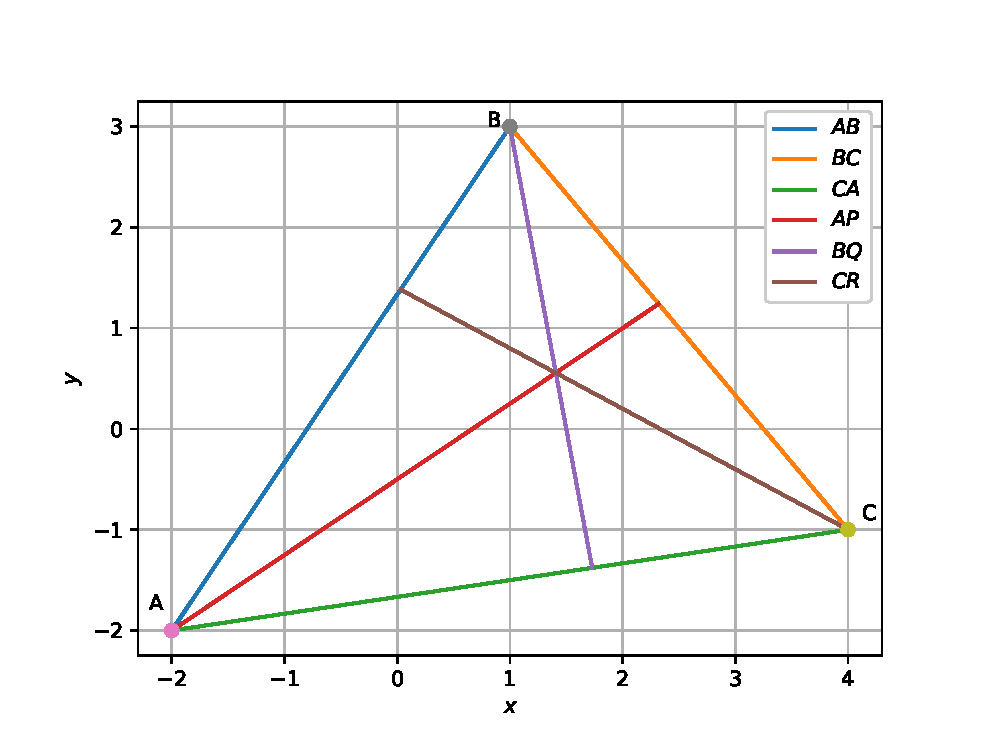
\includegraphics[width=\columnwidth]{./figs/alt_triangle.eps}
\caption{}
\label{fig:alt_triangle}
\end{figure}

\end{enumerate}
\section{Circumcircle}
%
\begin{enumerate}[label=\thesection.\arabic*
,ref=\thesection.\theenumi]

\item Let $\vec{A},\vec{B} $ and $\vec{C}$ be points on a circle with centre $\vec{O}$ and radius $r$.
\item Find $\vec{O}$.
\\
\solution The equation of the circle is 
\begin{align}
\label{eq:circle_def}
\norm{\vec{x}-\vec{O}} = R
\\
\implies \norm{\vec{x}-\vec{O}}^2 =\brak{\vec{x}-\vec{O}}^T\brak{\vec{x}-\vec{O}} = R^2
\end{align}
From \eqref{eq:circle_def},
\begin{align}
\label{eq:circle_AB}
\norm{\vec{A}-\vec{O}}^2 - \norm{\vec{B}-\vec{O}}^2  = 0
\end{align}
\begin{multline}
\implies \brak{\vec{A}-\vec{O}}^T\brak{\vec{A}-\vec{O}} 
\\
- \brak{\vec{B}-\vec{O}}^T\brak{\vec{B}-\vec{O}} = 0
\end{multline}
%
which can be simplified as
\begin{align}
\label{eq:circle_chord_ab}
\brak{\vec{A}-\vec{B}}^T\vec{O} =   \frac{\norm{\vec{A}}^2- \norm{\vec{B}}^2}{2}
\end{align}
Similarly,
\begin{align}
\label{eq:circle_chord_bc}
\brak{\vec{B}-\vec{C}}^T\vec{O} =   \frac{\norm{\vec{B}}^2- \norm{\vec{C}}^2}{2}
\end{align}
%
The following code computes $\vec{O}$ using the above two equations.
\begin{lstlisting}
https://raw.githubusercontent.com/gadepall/school/master/linalg/2D/python_2d/codes/circumcentre.py
\end{lstlisting}
\item Find the radius $R$.
\item Plot the {\em circumcircle} of $\triangle ABC$.
\\
\solution The following code plots Fig. \ref{fig:circumcircle}
\begin{lstlisting}
https://raw.githubusercontent.com/gadepall/school/master/linalg/2D/python_2d/codes/circumcircle.py
\end{lstlisting}
\begin{figure}
\centering
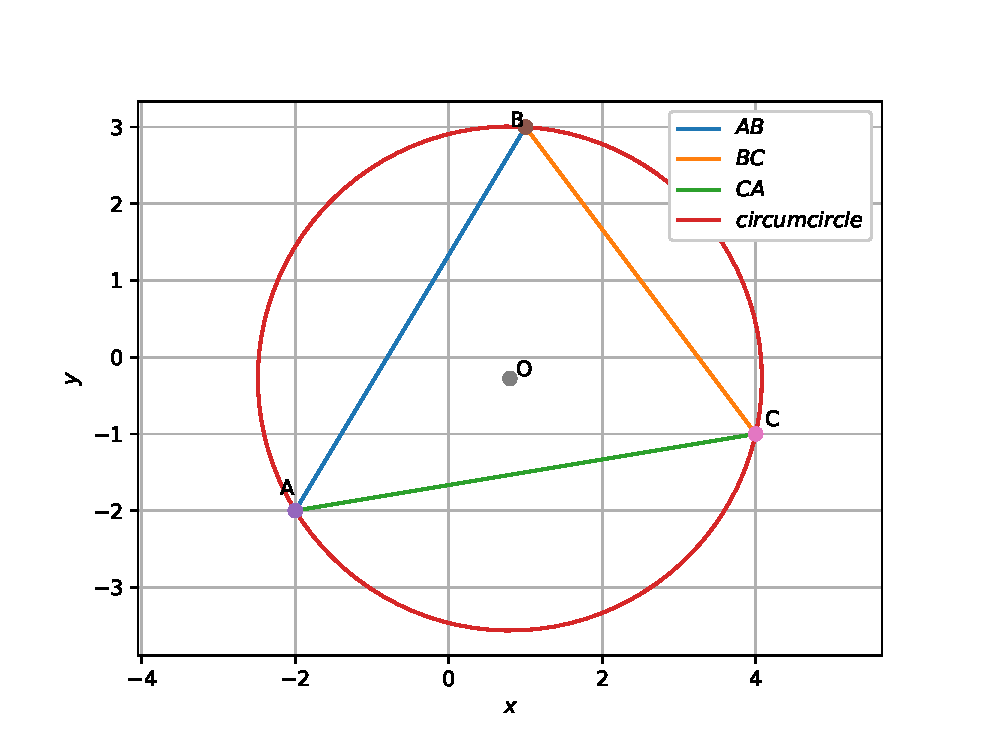
\includegraphics[width=\columnwidth]{./figs/circumcircle.eps}
\caption{}
\label{fig:circumcircle}
\end{figure}
\end{enumerate}

\section{Medians of a Triangle}
\begin{enumerate}[label=\thesection.\arabic*
,ref=\thesection.\theenumi]

\item
Find the coordinates of $\vec{D}, \vec{E}$ and $\vec{F}$ of the mid points of $AB, BC$ and $CA$ respectively 
for  $\Delta ABC$. 
%\\ 
%\solution
%The coordinates of the mid points are given by
%%
%\begin{align}
%D &= \frac{B+C}{2}, E = \frac{C+A}{2}, F = \frac{A+B}{2}
%\end{align}
%%
%The following code computes the values resulting in
%\begin{equation}
%D = \begin{pmatrix}
%2.5
%\\
%1
%\end{pmatrix},
%E = \begin{pmatrix}
%1
%\\
%-1.5
%\end{pmatrix},
%F = \begin{pmatrix}
%-0.5
%\\
%0.5
%\end{pmatrix},
%\end{equation}
%\lstinputlisting{./codes/mid_points.py}
\item
Find the equations of $AD,BE$ and $CF$. These lines are the {\em medians} of $\Delta ABC$
%\\
%\solution Use the code in Problem \ref{prob:line_eq}. 
%
\item
\label{prob:median}
Find the point of intersection of $AD$ and $CF$.
%\\
%\solution
%Let the respective equations  be
%\begin{align}
%\vec{n}_1^T\vec{x} &= p_1 \text{ and}
%\\
%\vec{n}_2^T\vec{x} &= p_2
%\end{align}
%This can be written as the matrix equation
%\begin{align}
%\myvec{ \vec{n}_1^T
%\\
%\vec{n}_2^T}
%\vec{x}
%&=
%\vec{p}
%\\
%\implies N^T \vec{x}
%&=
%\vec{p}
%\end{align}
%%
%where
%\begin{equation}
%N = \myvec{ \vec{n}_1 &
%\vec{n}_2},
%\end{equation}
%%
%The point of intersection is then obtained as
%\begin{align}
%\vec{x} &= \brak{N^T}^{-1}  \vec{p}
%\\
%&= N^{-T} \vec{p}
%\end{align}
%%
%The following code yields the point of intersection 
%\begin{equation}
%\vec{G} =
%\begin{pmatrix}
%1
%\\
%0
%\end{pmatrix}
%\end{equation}
%\lstinputlisting{./codes/line_intersect.py}
\item
%Using the code in Problem \ref{prob:median}, 
Verify that $\vec{G}$ is the point of intersection of $BE,CF$ as 
well as
$AD,BE$.  $\vec{G}$ is known as the {\em centroid} of $\Delta ABC$.
%\\
\item
Graphically show that the medians of $\Delta ABC$ meet at the centroid.
%\\
\item
Verify that
\begin{equation}
\vec{G} = \frac{\vec{A}+\vec{B}+\vec{C}}{3}
\end{equation}
\end{enumerate}
\section{Incircle}
%
\begin{enumerate}[label=\thesection.\arabic*
,ref=\thesection.\theenumi]

\item Consider a circle with centre $\vec{I}$ and radius $r$ that lies within $\triangle ABC$ and touches 
$BC, CA$ and $AB$ at $\vec{U}, \vec{V}$ and $\vec{W}$ respectively.

\item Show that $IU \perp BC$.
\\
\solution Let $\vec{x}_1,\vec{x}_2$ be two points on the circle such that 
$x_1x_2 \parallel BC$. Then
%
\begin{align}
\norm{\vec{x}_1-\vec{I}}^2- 
\norm{\vec{x}_2-\vec{I}}^2 &= 0 
\\
\implies 
\brak{\vec{x}_1-\vec{x}_2}^T\brak{\frac{\vec{x}_1+\vec{x}_2}{2}-\vec{I}} &= 
0 
\\
\implies 
\brak{\vec{B}-\vec{C}}^T\brak{\frac{\vec{x}_1+\vec{x}_2}{2}-\vec{I}} &= 
0 
%\label{eq:circle_bisect}
\end{align}
%
For $\vec{x}_1=\vec{x}_2=\vec{U}$, $x_1x_2$ merges into $BC$ and the above 
equation becomes 
%
\begin{align}
\brak{\vec{B}-\vec{C}}^T\brak{\vec{U}-\vec{I}} = 
0 
\implies OD \perp BC
%\label{eq:circle_bisect}
\end{align}
\item Find an expression for $r$ if $\vec{I}$ is known.
\\
\solution Let $\vec{n}$ be the normal vector of $BC$.  The equation for $BC$ is then given by
\begin{align}
\vec{n}^T\brak{\vec{x}-\vec{B}} &= 0
\\
\implies \vec{n}^T\brak{\vec{U}-\vec{B}} &= 0
\label{eq:incirc_ub}
\end{align}
since $\vec{U}$ lies on $BC$.
Since $IU \perp BC$, 
\begin{align}
\label{eq:incirc_iu}
\vec{I}&=\vec{U}+\lambda\vec{n}
\\
\implies \vec{I}-\vec{U}&=\lambda\vec{n}
\\
\text{or}\quad r=\norm{\vec{I}-\vec{U}}&=\abs{\lambda}\norm{\vec{n}}
\label{eq:incirc_r}
\end{align}
From \eqref{eq:incirc_ub} and \eqref{eq:incirc_iu}
\begin{align}
\vec{n}^T\vec{I}&=\vec{n}^T\vec{B}+\lambda\vec{n}^T\vec{n}
\\
\implies \vec{n}^T\brak{\vec{I}-\vec{B}}&=\lambda\norm{\vec{n}}^2
\\
\implies r = \abs{\lambda}\norm{\vec{n}}&=\frac{\abs{\vec{n}^T\brak{\vec{I}-\vec{B}}}}{\norm{\vec{n}}}
\end{align}
from \eqref{eq:incirc_r}.  Letting 
\begin{align}
\norm{\vec{n}_1}&= \frac{\vec{n}}{\norm{\vec{n}}},
\\
r &= \abs{\vec{n}_1^T\brak{\vec{I}-\vec{B}}}
\label{eq:incirc_rad}
\end{align}
\item Find $\vec{I}$.
\\
\solution Since $r = IU = IV = IW$, from \eqref{eq:incirc_rad},
\begin{align}
\abs{\vec{n}_1^T\brak{\vec{I}-\vec{B}}} = \abs{\vec{n}_2^T\brak{\vec{I}-\vec{C}}} = 
\abs{\vec{n}_3^T\brak{\vec{I}-\vec{A}}}
\label{eq:incirc_radeq}
\end{align}
%
where $\vec{n}_2, \vec{n}_3$ are unit normals of $CA, AB$ respectively.  \eqref{eq:incirc_radeq} can be 
expressed as 
\begin{align}
\vec{n}_1^T\brak{\vec{I}-\vec{B}} &= k_1\vec{n}_2^T\brak{\vec{I}-\vec{C}} 
\\
\vec{n}_2^T\brak{\vec{I}-\vec{C}} &= k_2\vec{n}_3^T\brak{\vec{I}-\vec{A}}
\label{eq:incirc_k1k2}
\end{align}
%
where $k_1,k_2 = \pm 1$. The above equations can be expressed as the matrix equation
\begin{align}
\myvec{\vec{n}_1-k_1\vec{n}_2 & \vec{n}_2 - k_2\vec{n}_3}^T\vec{I} &= 
\myvec{\vec{n}_1^T\vec{B}-k_1\vec{n}_2^T\vec{C} \\ \vec{n}_2^T \vec{C} - k_2\vec{n}_3^T\vec{A}}
\label{eq:incirc_k1k2fin}
\end{align}
\item Show that $\vec{I}$ lies inside $\triangle ABC$ for $k_1=k_2=1$
\item Compute $\vec{I}$ and $r$.
\\
\solution
\begin{lstlisting}
https://raw.githubusercontent.com/gadepall/school/master/linalg/2D/python_2d/codes/incentre.py
\end{lstlisting}
\item Plot the incircle of $\triangle ABC$
\\
\solution The following code plots the incircle in Fig. \ref{fig:incircle}
\begin{lstlisting}
https://raw.githubusercontent.com/gadepall/school/master/linalg/2D/python_2d/codes/incircle.py
\end{lstlisting}
\begin{figure}
\centering
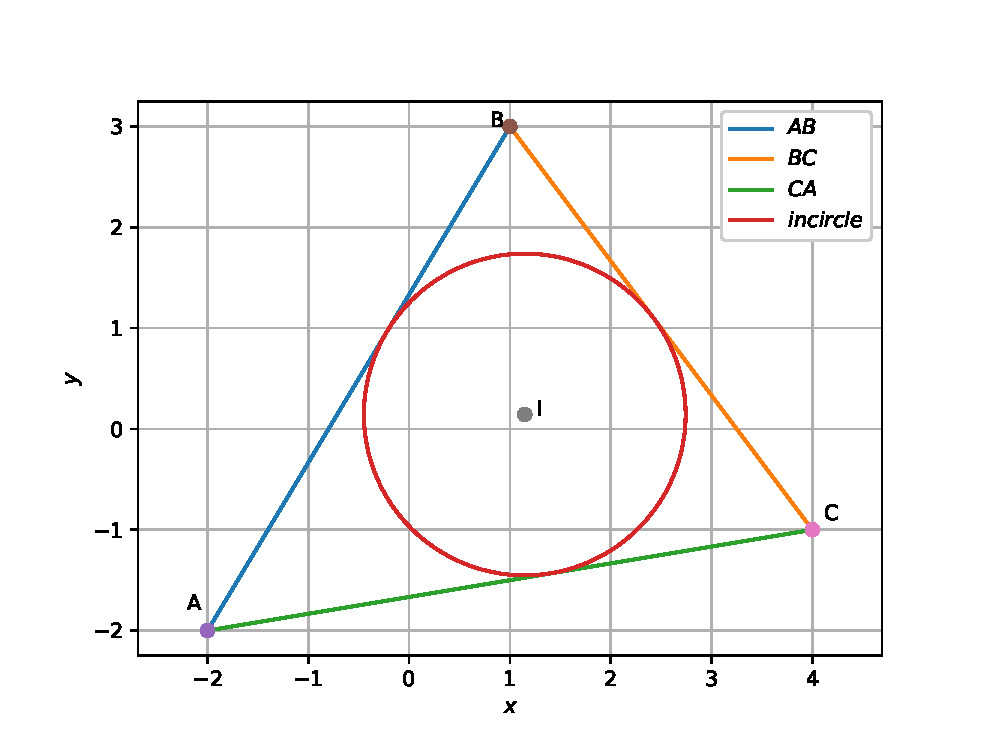
\includegraphics[width=\columnwidth]{./figs/incircle.eps}
\caption{}
\label{fig:incircle}
\end{figure}

\end{enumerate}
\end{document}


